\chapter{Learning from complex vehicle model}
\label{cha:Tracking_MPC}

%Plot simulink model en duidt de blokken aan die zullen worden ingevuld. Hier gaat dieper in gegaan worden in de volgende hoofdstukken. 

Because the non-linear bicycle model makes abstraction of dynamics that are applicable in a real vehicle, a more complex model is introduced in order to improve the reality factor of the simulations. In order to achieve this the $15$ degrees of freedom amesim model as can be seen in Figure \ref{fig:Amesim}, is provided by Siemens. The parameters of this model are tuned by the company in order to behave similar to a testcar they are currently using. The model has as inputs the amount of throttle, braking and a steerwheelangle.  

\begin{figure}[h!]
	\centering
	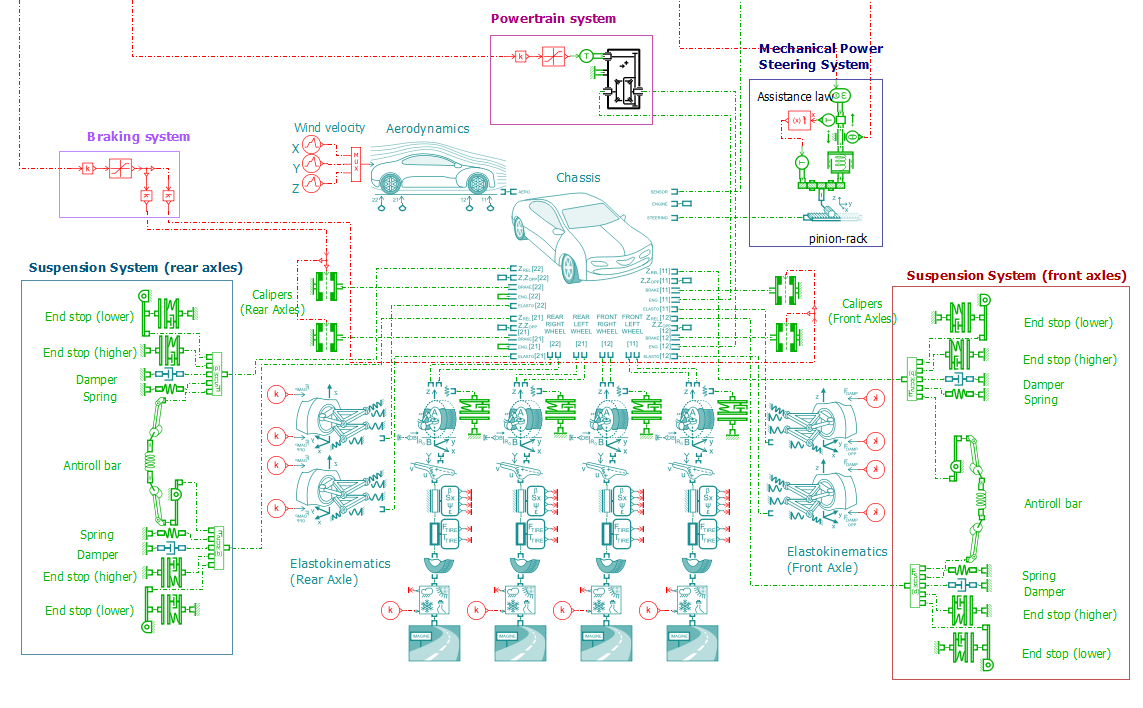
\includegraphics[width=1.0\textwidth]{Amesim.PNG}
	\caption{The 15 dof amesim model with as inputs the amount of throttle, braking and steerwheelangle.}	
	\label{fig:Amesim}
\end{figure}

The Amesim model serves as a black box and no direct dynamic equations are available 
to include in \ref{opt:basic_opti_w} as was done with the non-linear bicycle model \ref{eq:bicycle_model_eqmotion}. Therefore a path is planned with the simpler non-linear bicycle model and afterwards a model predictive control tracking algorithm is applied on the Amesim model in order to follow its reference. The working principles of a MPC is discussed in \ref{s:MPC_e}. Diagram \ref{fig:complex_learning} shows the flow of handlings that is done during learning with the Amesim model.

\begin{figure}[h!]
	\centering
	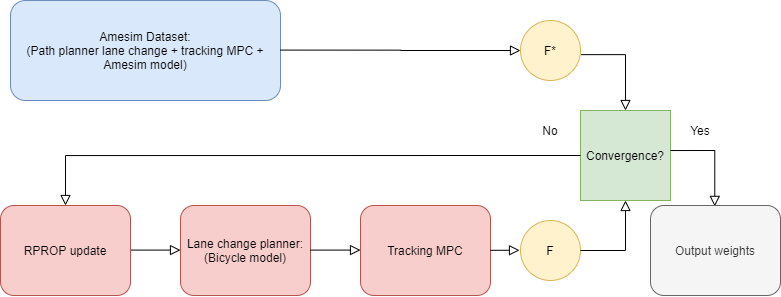
\includegraphics[width=1.1\textwidth]{complex_learning_diagram.PNG}
	\caption{The flow of learning with the Amesim model.}	
	\label{fig:complex_learning}
\end{figure}

As is described in Diagram \ref{fig:complex_learning} the feature vector $\bm{F}(\bm{r})$ is also calculated based on the Amesim model and used in the convergence block to calculate the estimation of the gradient by $\pdv{\bm{F}}{\bm{\theta}} = \bm{F}_{obs} - \bm{F}(\bm{r}_{expected})$. The reason for this is to avoid to integrate the vehicle mismatch between the non-linear bicycle model and the Amesim model into the learned path. This concretely means that it otherwise is possible that even when the learning algorithm is capable to match the feature vectors $\bm{F}(\bm{r})$ and  $\bm{F}^*(\bm{r})$, coming form two different vehicle models, the learned kinematic signals of the bicycle model will not represent the observations accurate enough. In order to check this, table \ref{tab:comparinson_models} \footnote{Note that the feature values of the bicycle model are slightly different values than the ones in table \ref{tab:GD_local_test}. This is because in the previous table the time limit was set on $30 \hspace{1mm}s$ and here time limit is $30 \hspace{1mm}s$. This is done to have a better useable time discretization of $0.025\hspace{1mm}s$ to input to the Amesim model.} shows the difference of feature values for a lane change $V_0:22.22\hspace{1mm}\frac{m}{s},\hspace{1mm} L:3.47\hspace{1mm}m$ generated with the non-linear bicycle model and afterwards tracked with the Amesim model.\\

\newpage

\begin{table}[h!]
	\centering
	\begin{tabular}{@{}llr@{}} \toprule
		Feature Value    & Bicycle model & Amesim model\\ \midrule
		Nr.1       		 & 5.28e-8    & 3.33e-7 \\
		Nr.2       		 & 0.37       & 0.38  \\
		Nr.3       		 & 1.41e-7    & 1.20e-4 \\
		Nr.4       		 & 0.57       & 0.49  \\
		Nr.5       		 & 1.89e-6    & 9.40e-6 \\
		Nr.6       		 & 30.99      & 31.05\\ \bottomrule
	\end{tabular}
	\caption{This table shows the feature values obtained of a lane change $V_0:22.22\hspace{1mm}\frac{m}{s},\hspace{1mm} L:3.47\hspace{1mm}m$ for respectively the Bicycle and Amesim model.}
	\label{tab:comparinson_models}
\end{table}

As can be seen the features of the reference produced by the bicycle model are almost the same as the ones that are retrieved from the Amesim model during the application of the tracking MPC. However not all kinematic signals give an accurate match as is described in Appendix \ref{app:D} and further discussed in section \ref{s:tracking_mpc}. 

This chapter also gives an answer on the question if the estimate of the gradient $\pdv{\bm{F}}{\bm{\theta}}$ by $ \bm{F}_{obs} - \bm{F}(\bm{r}_{expected})$ is still sufficient in order to match the learned and observed feature values in section \ref{s:complex_learning_results}.

\section{Tracking MPC} 
\label{s:tracking_mpc}
To be able to integrate the Amesim model in the learning process in an adequate manner, good tracking is desirable for the important features that determine the lane change planning. For the lane change maneuver looked at in this thesis, a good tracking is therefore wanted for: $y(t), a_y(t)$ and $j_y(t)$.

\subsection{MPC formulation}
The tracking is achieved by making use of the non-linear bicycle model defined with 10 states as defined in \ref{eq:bicycle_model2} inside the OCP formulation given by $\ref{opt:tracking}$ that is called during the MPC loops. The control horizon of the MPC is $N_{MPC}$ and equal to $50$ points which means a control horizon of $1.25 \hspace{1mm}s$ because the reference is sampled with $T_{pl}$ equal to $0.025\hspace{1mm}s$. The parameters of the bicycle model stay the same as the ones listed in \ref{table:vehicel_model_param}. The objective function used is the error function between the reference states and the states visited during the control horizon starting from the current state. In order to define the gap closing constraint, which means connecting the previous states to the next in this multiple shooting formulation, Runge-Kutta integration is embedded in function $I$.  
The first time that the OCP is solved and the current state is not yet outputted by the sensors on the Amesim model, the initial states are set equal to its first reference point. The path constraints can be seen in \ref{eq:F_MPC} and the error function $E(\bm{X}(.),\bm{U}(.))$ that serves as objective is shown in \ref{eq:obj_mpc}.


\begin{equation}\label{opt:tracking}
\begin{aligned}
\min_{\bm{X}(.),\bm{U}(.)} \quad &  E(\bm{X}(.),\bm{U}(.)) \\
\textrm{s.t.} \quad & \bm{X}^{k+1} = I(\bm{X}^{k}, \bm{U}^{k}) & k = [0,\cdots, N_{MPC}-1]\\
& \bm{X}^{0} = \bm{X}_{intitial} \\
& \bm{F}(\bm{X}^{k}) \geq 0	& k = [0,\cdots, N_{MPC}]\\
& \bm{X}^{k}\in \mathbb{R}^{10\times 1}  & k = [0,\cdots, N_{MPC}]\\
& \bm{U}^{k}\in \mathbb{R}^{2\times 1} \hspace{3 mm} & k = [0,\cdots, N_{MPC}-1]\\
&  N_{MPC} \in \mathbb{N}
\end{aligned}
\end{equation}

The path constraints shown in \ref{eq:F_MPC} are at first sight not necessary but contribute by decreasing the feasible solution space for the solver in \ref{opt:tracking}. It is checked that these constraints are not binding, which means that the found solution is reachable even if the constraints were removed. 

\begin{equation}\label{eq:F_MPC}
\bm{F} =
\begin{Bmatrix}
-\frac{Width\hspace{1mm}Lane}{2} \leq y^k \leq \frac{3\cdot Width\hspace{1mm}Lane}{2}, & k = [0,\cdots, N_{MPC}] \\
0 \leq x^k, & k = [0,\cdots, N_{MPC}] \\
-\frac{\pi\cdot 5}{180} \leq \psi^k \leq \frac{\pi\cdot 5}{180}, & k = [0,\cdots, N_{MPC}] \\
v_{start}-1 \leq v_x^k \leq v_{start}+1, & k = [0,\cdots, N_{MPC}]
\end{Bmatrix}
\end{equation}\

The error function that serves as the objective of the OCP is given by the following equation. The weights that gave the best tracking results can be seen in table \ref{tab:weights}.

\begin{multline*} 
objective=W_1(\bm{x}[2:end]-\bm{ref}_x)^T(\bm{x}[2:end]-\bm{ref}_x)+W_2(\bm{y}[2:end]-\bm{ref}_y)^T(\bm{y}[2:end]-\bm{ref}_y)\\
+W_3(\bm{v}_x[2:end]-\bm{ref}_{v_x})^T(\bm{v}_x[2:end]-\bm{ref}_{v_x})+W_4(\bm{v}_y[2:end]-\bm{ref}_{v_y})^T(\bm{v}_y[2:end]-\bm{ref}_{v_y})\\+W_5(\bm{\psi}[2:end]-\bm{ref}_{\psi})^T(\bm{\psi}[2:end]-\bm{ref}_\psi)
+W_6(\bm{\dot{\psi}}[2:end]-\bm{ref}_{\dot{\psi}})^T(\bm{\dot{\psi}}[2:end]-\bm{ref}_{\dot{\psi}})\\ + W_7\dot{\bm{t}}_r^T\dot{\bm{t}}_r+W_8\dot{\bm{\delta}}_s^T\dot{\bm{\delta}}_s + W_9\dot{\bm{a}}_x^T\dot{\bm{a}}_x
\end{multline*}

\[\bm{x},\bm{y},\bm{v}_x,\bm{v}_y,\bm{\psi},\dot{\bm{\psi}},\bm{a}_x \in \mathbb{R}^{(N_{MPC}+1)\times1} \hspace{10mm}\bm{ref}_{i},\dot{\bm{t}}_r,\dot{\bm{\delta}}_s \in \mathbb{R}^{N_{MPC}\times1}\]


\begin{table}[h!]
	\centering
	\begin{tabular}{@{}lr@{}} 
		Weight    & Value\\ \midrule
		W1      & 10\\
		W2          & 10\\
		W3 	   & 30\\
		W4       & 1.0\\
		W5       & 100\\
		W6       & 1.0\\
		W7       & 5.0\\
		W8       & 0.01\\
		W9  & 0.01\\ \bottomrule
	\end{tabular}
	\caption{Overview of the weights used in the objective of \ref{opt:tracking}.}
	\label{tab:weights}
\end{table}

The ultimate weights displayed were attained by trail and error but there is an intuitive explanation on why these states were used and which order of magnitude the weights were given.\\
It was first tried to focus mostly on path tracking in order to see how the other states would differ when the Amesim model drove almost exactly the same path as the non-linear vehicle and therefore $x(t),y(t)$ and $\psi(t)$ were included. They define the orientation of the vehicle. Nervous input behaviour was noticed and in order to smooth the input they were given a small weight. This in order assure still good tracking behaviour. It was observed that this strategy resulted in a good tracking of the important signals for the learning algorithm: $y(t), a_y(t)$ and $j_y(t)$. As will be explained in \ref{s:tracking_results} at the start of the maneuver the Amesim model made a deceleration. In order to  give the model time to stabilize before the start of the maneuver, a straight driving part of $15\hspace{1mm}s$ and $2.5\hspace{1mm}s$ were respectively added before and after the reference lane change maneuver. To faster remove the oscillation in the longitudinal direction of the vehicle, $v_x$ and $a_x$ were included in the objective.\\

The initial guess given to first solve the OCP is only needed for $v_x$. This is because otherwise an invalid value would emerges in the calculation of the slipangle according to equation \ref{eq:bicycle_slipangle}. When the OCP is defined and implemented in CasADi as described above, the opti environment is saved as a function that can be called during the running of the MPC. In order to speed up the implementation there is switched to a SQP method using an active-set QP solver instead of IPOPT that was used in \ref{opt:basic_opti_w}. "Interior point methods (like IPOPT) are generally robust at finding a minimizer, but the barrier parameter will make the algorithm walk away from a perfect initial guess, only to come back after a while." \cite{Gillis2019} A hot starting was implemented by feeding the solution of a previous MPC iteration as initial guess for the optimization variables and the lambda multipliers. Because of this it was logical to switch the solver and solving method. Together with the straight driving parts, a simulation of $40\hspace{1mm}s$ is performed and one iteration of the MPC takes around $0.15\hspace{1mm}s$. The main time consumed to calculate the solution is mainly the loading time needed for the different simulation components.\\

With the OCP defined, it can be included in a MPC formulation. Every MPC iteration the current state is outputted by the Amesim model and the reference which are implemented as parameters the optimization \ref{opt:tracking}. The Amesim model is evaluated at a sampling rate of $T_s$ and the optimization \ref{opt:tracking} outputting controls is called at a rate of $T_{MPC} = 0.1$.\footnote{It can be noted that the reference comes at a sampling rate $T_{pl}$ of $0.025\hspace{1mm}s$ which is taken into account during the reference update.}  In order to connect the tracking MPC with the Amesim model using different sampling times, the Simulink model of Figure \ref{fig:simulink_model} was build. 

\begin{figure}[h!]
	\centering
	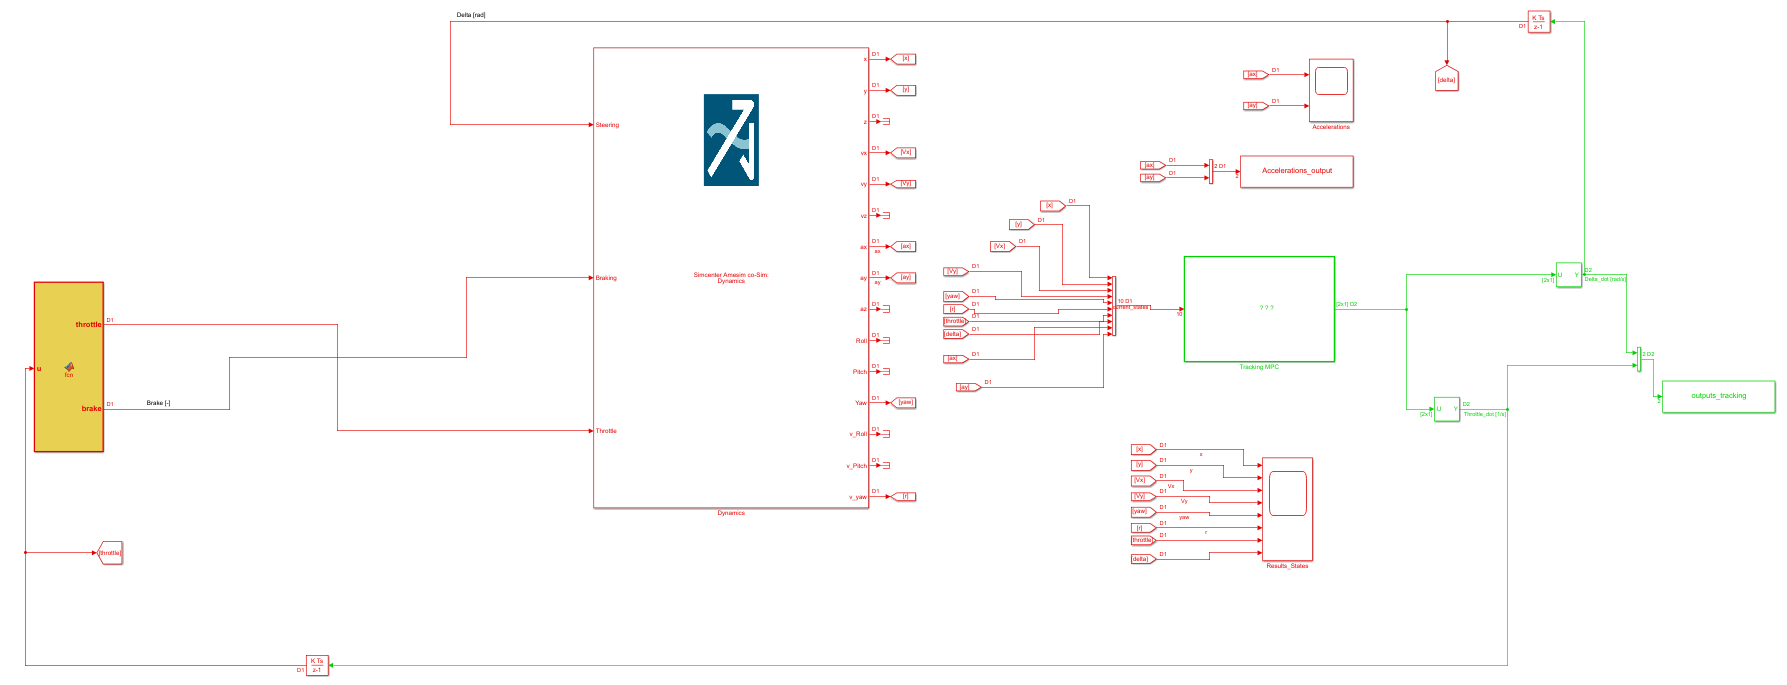
\includegraphics[width=1.1\textwidth]{simulink_model.PNG}
	\caption{This figure shows hows the tracking MPC is connected with the Amesim model using different sampling times. (red: $T_s: 0.01\hspace{1mm}s$ and green: $T_{MPC}:0.1\hspace{1mm}s$)}	
	\label{fig:simulink_model}
\end{figure}

The three inputs to the Amesim model (largest block) are $\delta_s$, $t_r$ and $braking$ but the control outputs of \ref{opt:tracking} give $\dot{t}_r$ and $\dot{\delta_s}$. Therefore 'Forward Euler integration' was introduced using for $0.1\hspace{1mm}s$ the control outputs in order to calculate every $0.01\hspace{1mm}s$ the inputs for the Amesim model. Moreover the throttle of the bicycle model can theoretically become positive and negative. These two states were separated and feeded to the Amesim model as throttling or braking. 


\subsection{Tracking results} 
\label{s:tracking_results}

In this section the results of the tracking MPC are displayed. For a full overview of the results, reference is made to Appendix \ref{app:D}. Figure \ref{fig:xy_mpc} shows that the tracking of the path (blue) of the reference (red) is done with an accuracy of $10^{-3}$. 

\begin{figure}[h!]
	\centering
	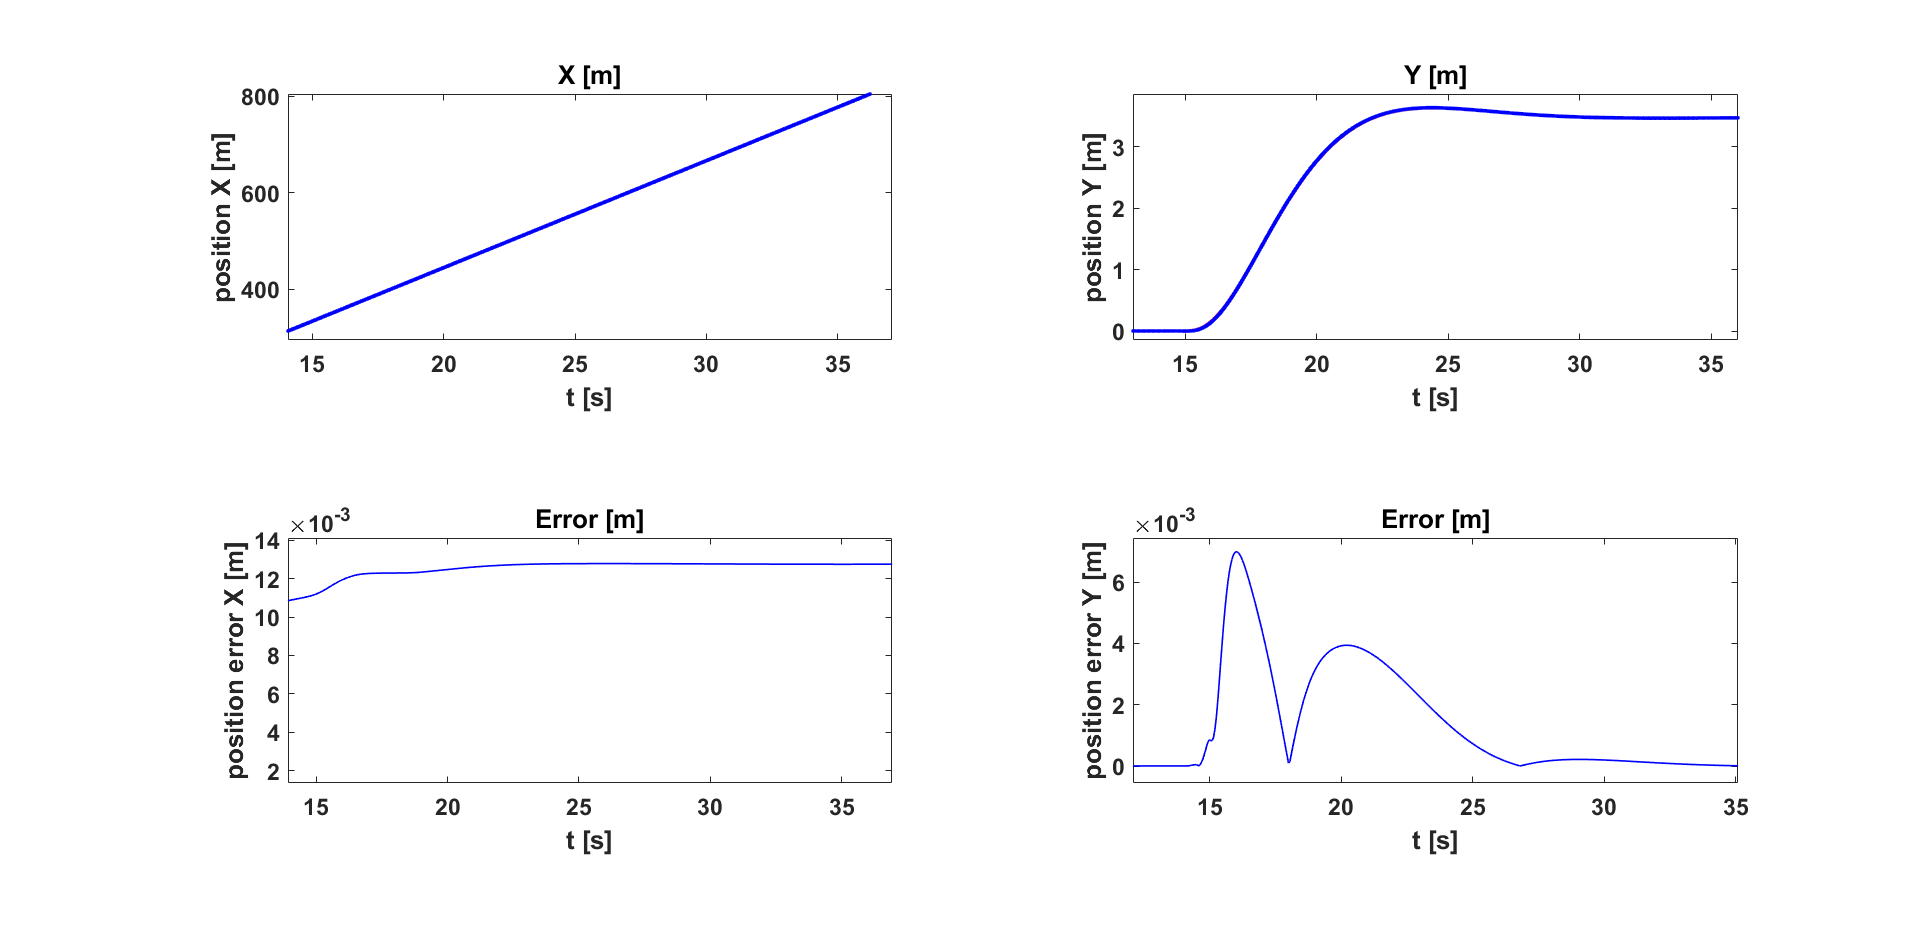
\includegraphics[width=1.15\textwidth]{2xy_N50_TMPC 0.1_Tf40.PNG}
	\caption{This figure shows the tracking result of the reference (red) by the Amesim model (blue).}	
	\label{fig:xy_mpc}
\end{figure}

During the analysing of the results it was concluded that the important signals were followed sufficiently well in order to use the MPC for learning in a configuration as is shown by Figure \ref{fig:complex_learning}. However there were also differences seen between the reference and the followed trajectory. This justifies the reasoning that not all states have to be included in the error function of \ref{opt:tracking}, because tracking all states accurate will give worse results due to inherent vehicle model mismatch. Firstly the Amesim model needs a bigger steerwheelangle than was predicted by the reference. Also the amount of throttle needed to drive forward at a constant speed is slightly different because of the more complete way of aerodynamic resistance modelled by the Amesim model in comparison to equation \ref{eq:bicycle_Fdrag}.\\
Another interesting observation was that the lateral jerk and first derivative of the steerwheelangle display less high peaks than the reference model. If very closely zoomed in on the longitudinal jerk around $15\hspace{1mm}s$ which coincides with the start of the lane change and $22\hspace{1mm}s$, which is more at the end, nervous behaviour of the longitudinal jerk is witnessed. Around $15\hspace{1mm}s$ also a bump in the reference of the throttle can be seen because that is the point that straight driving at constant speeds ends and the reference is from that point produced by solving \ref{opt:basic_opti_w}. The influence on $v_x$ and $a_x$ is however marginal. Further it is good to note that the jerks don't come directly from the Amesim model but the signal is post-processed by numerical differentiation. \\

To be able to generate adequately smooth jerk signals, it was necessary to include smooth enough inputs of throttle and steerwheelangle. Figure \ref{fig:old_inputs} shows the cycling of the jerk that is obtained when not the first derivative of throttle and steerwheelangle is applied as input to the Amesim model. That the jerk signal is dependent on the first derivative of the throttle and steeringwheelangle is a logical result, because also in the analytical jerk equations of the non-linear bicycle model (appendix \ref{app:A}) these variables were included.\footnote{For this result no straight driving reference path is added. The lane change start directly at $time = 0.0$.}

\begin{figure}[h!]
	\centering
	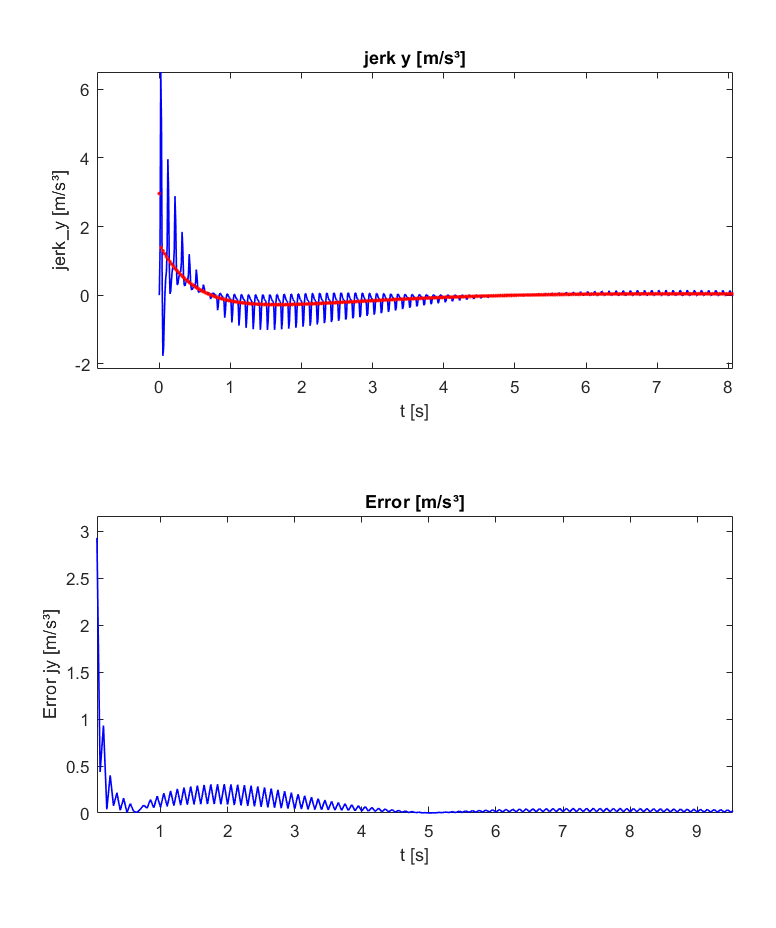
\includegraphics[width=0.8\textwidth]{9jerks_N50_TMPC 0.1_Tf22.5_adjusted.PNG}
	\caption{This figure shows the obtained oscillating signals for the jerk when a piecewise signal of $\delta_s$ and $t_r$ is applied.}	
	\label{fig:old_inputs}
\end{figure}

\section{Learning results with the Amesim model}
\label{s:complex_learning_results}
Diagram \ref{fig:complex_learning} shows in blue the observed path that is generated out of \ref{opt:basic_opti_w} with known weights whereafter the path based on a bicycle model is tracked by a tracking MPC to get the kinematic signals of the $15$ dof Amesim model. From this $\bm{F}^*(\bm{r})$ is calculated which stays constant during whole the learning process.\\

The learning loop shown in red in diagram \ref{fig:complex_learning} starts at the lane change planner, where \ref{opt:basic_opti_w} is called with as initial guess of the weights an all one vector. After the planned path that was outputted by the planner, is tracked and the feature vector $\bm{F}(\bm{r})$ is calculated, it is checked if the two feature vectors match in the convergence block. If this is not the case, the difference of the features is taken as an estimate for $\pdv{\bm{F}}{\bm{\theta}}$ and used in the RPROP algorithm in order to generate a new planned path by calling \ref{opt:basic_opti_w}. The first $10 \hspace{1mm}s$ of the tracked Amesim signal is removed.\\
Three simulations are conducted with respectively one, two and three datasets. Table \ref{tab:datasets_overview} shows which longitudinal speed is driven at the begin of the lane change ($V_{0}$) and the lateral displacement of the driver $(L)$. As is noted before in Chapter $\ref{cha:Learning_algorithm}$, if only the start speed is varied, the lateral feature values stay the same and the longitudinal features stay very small, which means that these datasets are seen as almost the same when learning. When the lateral desired displacement is varied, this gives a clear difference in the lateral feature values. An overview of the different features of the individual datasets is given in table \ref{tab:indi_features}. \footnote{In the calculation of the feature values the $5 \hspace{1mm}s$ straight driving before the lane change is included. This contributes to bigger number six feature values.} 



\begin{table}[h!]
	\centering
	\begin{tabular}{@{}llllr@{}} \toprule
		1 Dataset    & 2 Datasets & 3 Datasets\\ \midrule
     $V0:22.22 - L:3.47$  & $V0:22.22 - L:3.47$    & $V0:22.22 - L:3.47$ 		\\
           			 & $V0:25.00 - L:6.94$      & $V0:25.00 - L:6.94$      \\
	        		 &        & $V0:27.78 - L:3.47$      \\ \bottomrule
	\end{tabular}
	\caption{This table shows which lane changes were used during the three different simulations.}
	\label{tab:datasets_overview}
\end{table} 


\begin{table}[h!]
	\centering
	\begin{tabular}{@{}llllr@{}} \toprule
	\textbf{Feature Value}     & V022.22 - L3.47 & V025.00 - L6.94 & V027.78 - L3.47\\ \midrule
		Nr.1       		  &5.18e-07       & 5.97e-06  & 4.01e-07 		\\
		Nr.2              & 0.38       & 1.51       & 0.38       \\
		Nr.3              & 12.29e-05  & 7.23e-05      & 5.37e-06      \\
		Nr.4              & 0.51       & 2.09       &   0.52    \\
		Nr.5              & 9.50e-06       & 7.08e-05       & 3.71e-05       \\
		Nr.6              & 91.25      & 364.97       & 91.25       \\ \bottomrule
	\end{tabular}
	\caption{This table shows the different features for the individual datasets used during simulation.}
	\label{tab:indi_features}
\end{table} 

The weights found for the three different simulations are presented in table \ref{tab:complex_learning_weights} and the $\bm{f}_{rel}$ values are given in table \ref{tab:complex_frel}.  $\bm{f}_{rel}$ displays the matching of the averaged learned feature values with the observed one. Convergence was for the three simulations reached after 28 iterations. The convergence criteria used is matching of the lateral features (2,4,6) with a tolerance of $10^{-3}$.

\begin{table}[h!]
	\centering
	\begin{tabular}{@{}llllr@{}} \toprule
		\textbf{Weight}   & 1 Dataset    & 2 Datasets     & 3 Datasets\\ \midrule
		Nr.1       		  &33.4230       & 5.2294       & 3.9036		\\
		Nr.2              & 5.0000         & 5.0000          & 5.0000       \\
		Nr.3              & 2.8662e-06     & 1.0636      & 1.9803      \\
		Nr.4              & 6.0018           & 6.0018            &   6.0018     \\
		Nr.5              & 4.4445     & 1.2705      & 1.1869       \\
		Nr.6              & 2.0011        & 2.0011         & 2.0011      \\ \bottomrule
	\end{tabular}
	\caption{This table shows the weights learned for the different simulations that start from an all one vector and uses as chosen weights $\bigl[ \begin{smallmatrix} 4.0,&5.0,&1.0,&6.0,&1.0,&2.0\end{smallmatrix}\bigr]$.}
	\label{tab:complex_learning_weights}
\end{table}

\begin{table}[h!]
	\centering
	\begin{tabular}{@{}llllr@{}} \toprule
		$\bm{f}_{rel}$   & 1 Dataset    & 2 Datasets     & 3 Datasets\\ \midrule
		Nr.1       		  &1.1315        & 1.0097       & 0.9643		\\
		Nr.2              & 1.0000         & 1.0002     & 1.0003       \\
		Nr.3              & 0.2865     & 0.4496     	& 0.4867      \\
		Nr.4              & 1.0000           & 1.0002   &   1.0002     \\
		Nr.5              & 1.0718     & 1.0030         & 0.9937       \\
		Nr.6              & 1.0000        & 1.0000      & 1.0000     \\ \bottomrule
	\end{tabular}
	\caption{This table shows the final values of $\bm{f}_{rel}$.}
	\label{tab:complex_frel}
\end{table}

Out of table \ref{tab:complex_learning_weights} and \ref{tab:complex_frel} it follows that the lateral chosen weights are found back and an accurate match of the lateral features is achieved. It is observed that also the longitudinal weights will come closer to their chosen value and give a better match of the longitudinal feature values, when more observed lane changes are included in the learning.\\

Figure \ref{fig:complex_path} presents the observed paths, the initial solution when the weight vector is chosen equal to an all-one vector and the learned solution when $2$ datasets are used. Figure \ref{fig:complex_path_error} shows the error made between the observed and learned path which has order of size of $10^{-4}$.

\begin{figure}[h!]
	\centering
	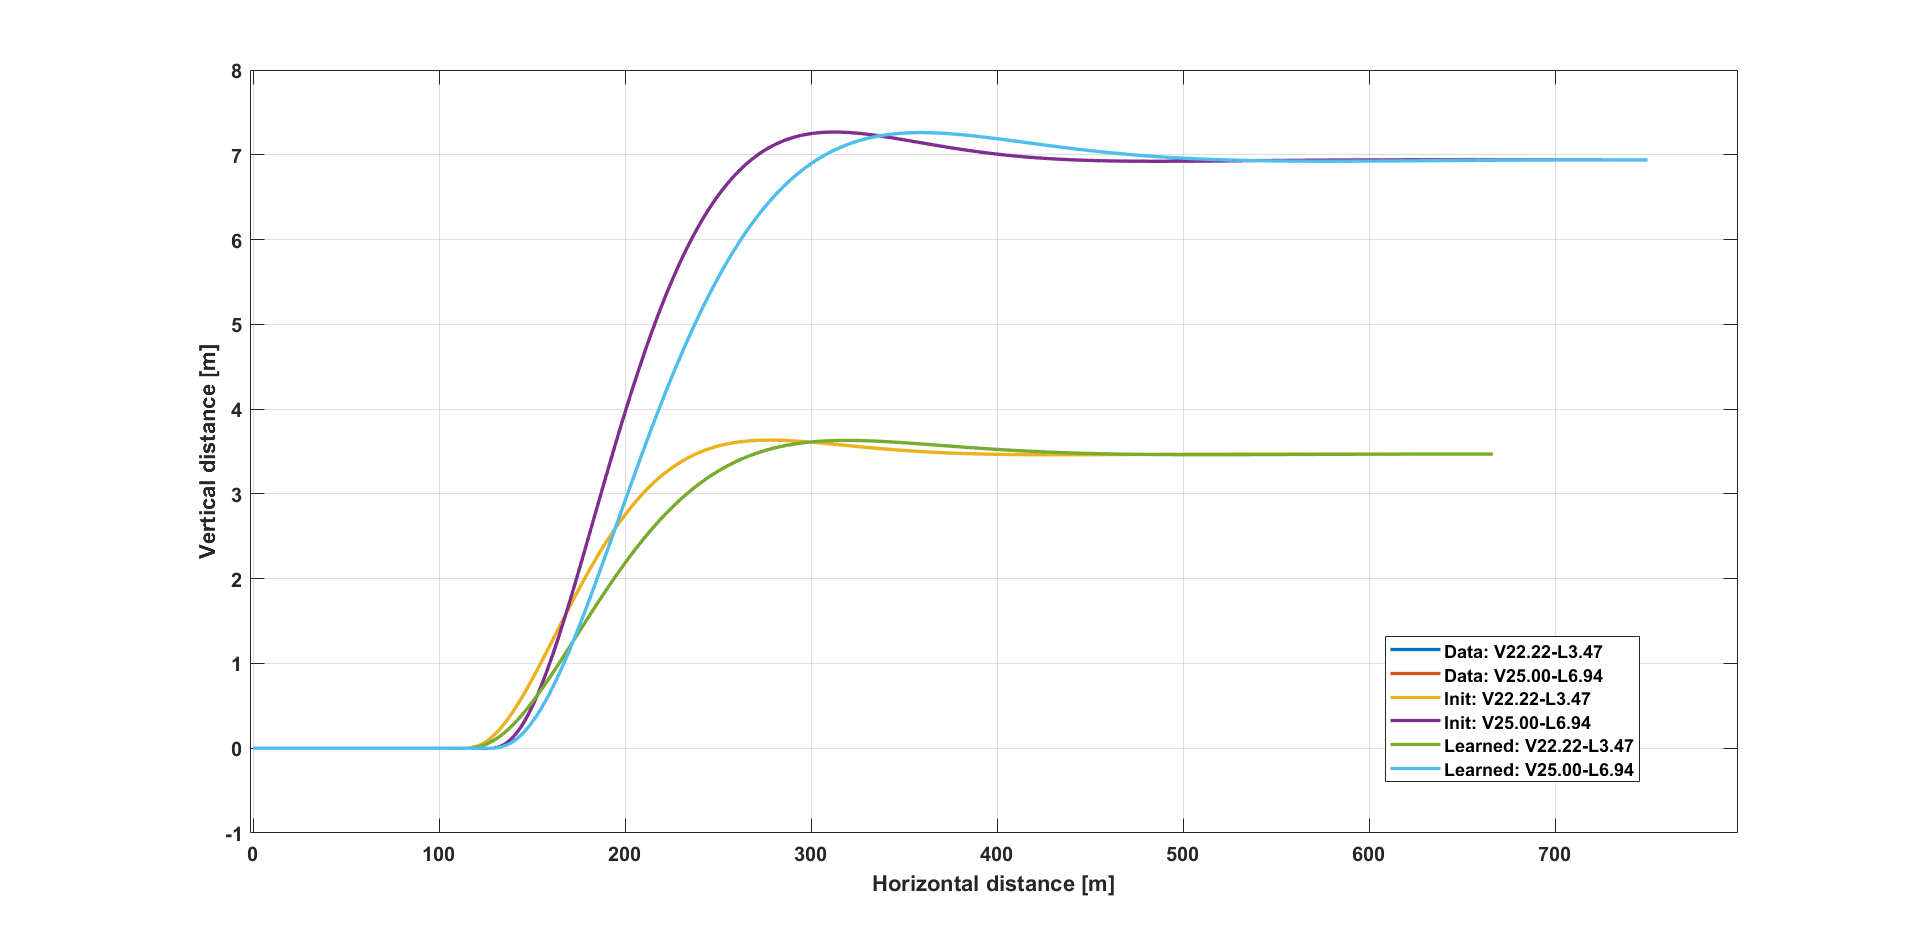
\includegraphics[width=1.1\textwidth]{2path_N1000IT28.PNG}
	\caption{This Figure shows the observed paths, the initial solution retrieved with as weights an all one vector and the learned solution.}	
	\label{fig:complex_path}
\end{figure}

\begin{figure}[h!]
	\centering
	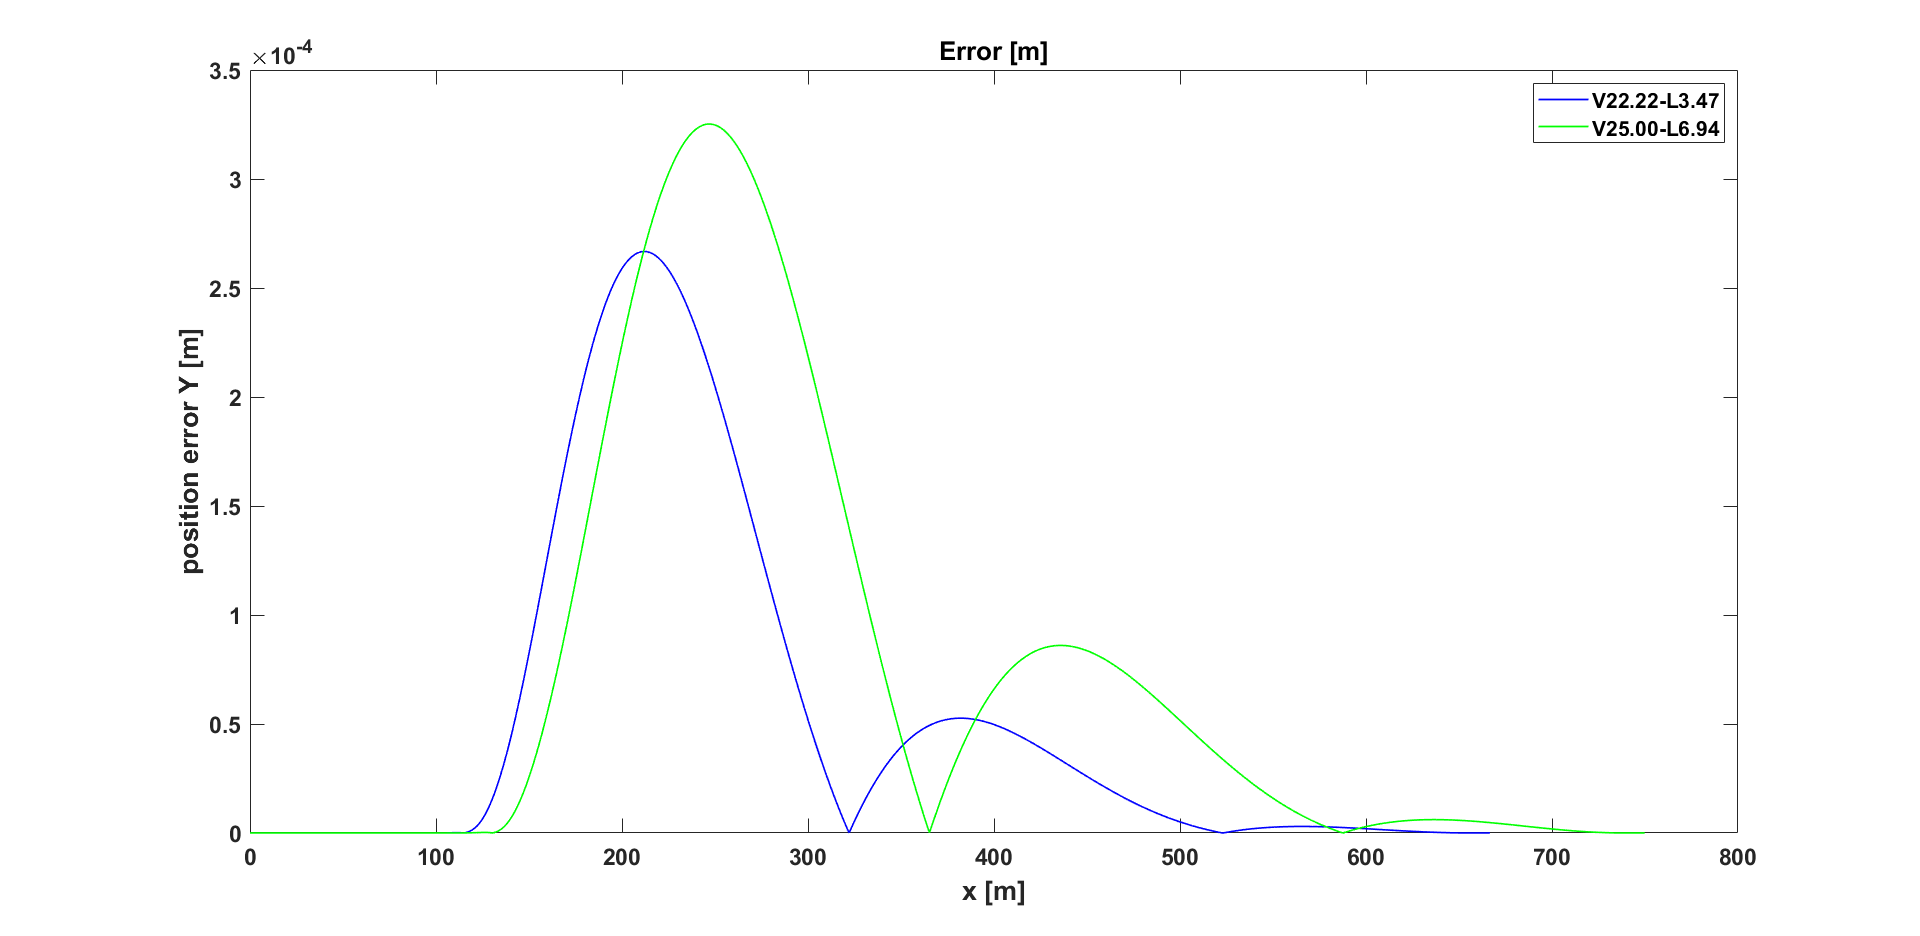
\includegraphics[width=1.1\textwidth]{error learned path.PNG}
	\caption{This Figure shows the observed paths, the initial solution retrieved with as weights an all one vector and the learned solution.}	
	\label{fig:complex_path}
\end{figure}

Figure \ref{fig:complex_convergence} shows the convergence of $\bm{f}_{rel}$ towards one during the learning iterations. 



From all the retrieved $\bm{f}_{rel}$ of table \ref{tab:complex_frel} and in Figure \ref{fig:complex_convergence} the feature value for the longitudinal jerk (Nr. $3$), jumps out for its bad feature matching behaviour. (only $0.4867$ when three datasets are used) A reason for this is as discussed in \ref{s:tracking_results} bad quality of the jerk data which contributes to a worse learning.The figure of the jerk during the lane change can be seen in Figure \ref{fig:complex_jerk}. At time zero the longitudinal behaviour is still not fully stabilized and at second $5$ the lane change starts.

\begin{figure}[h!]
	\centering
	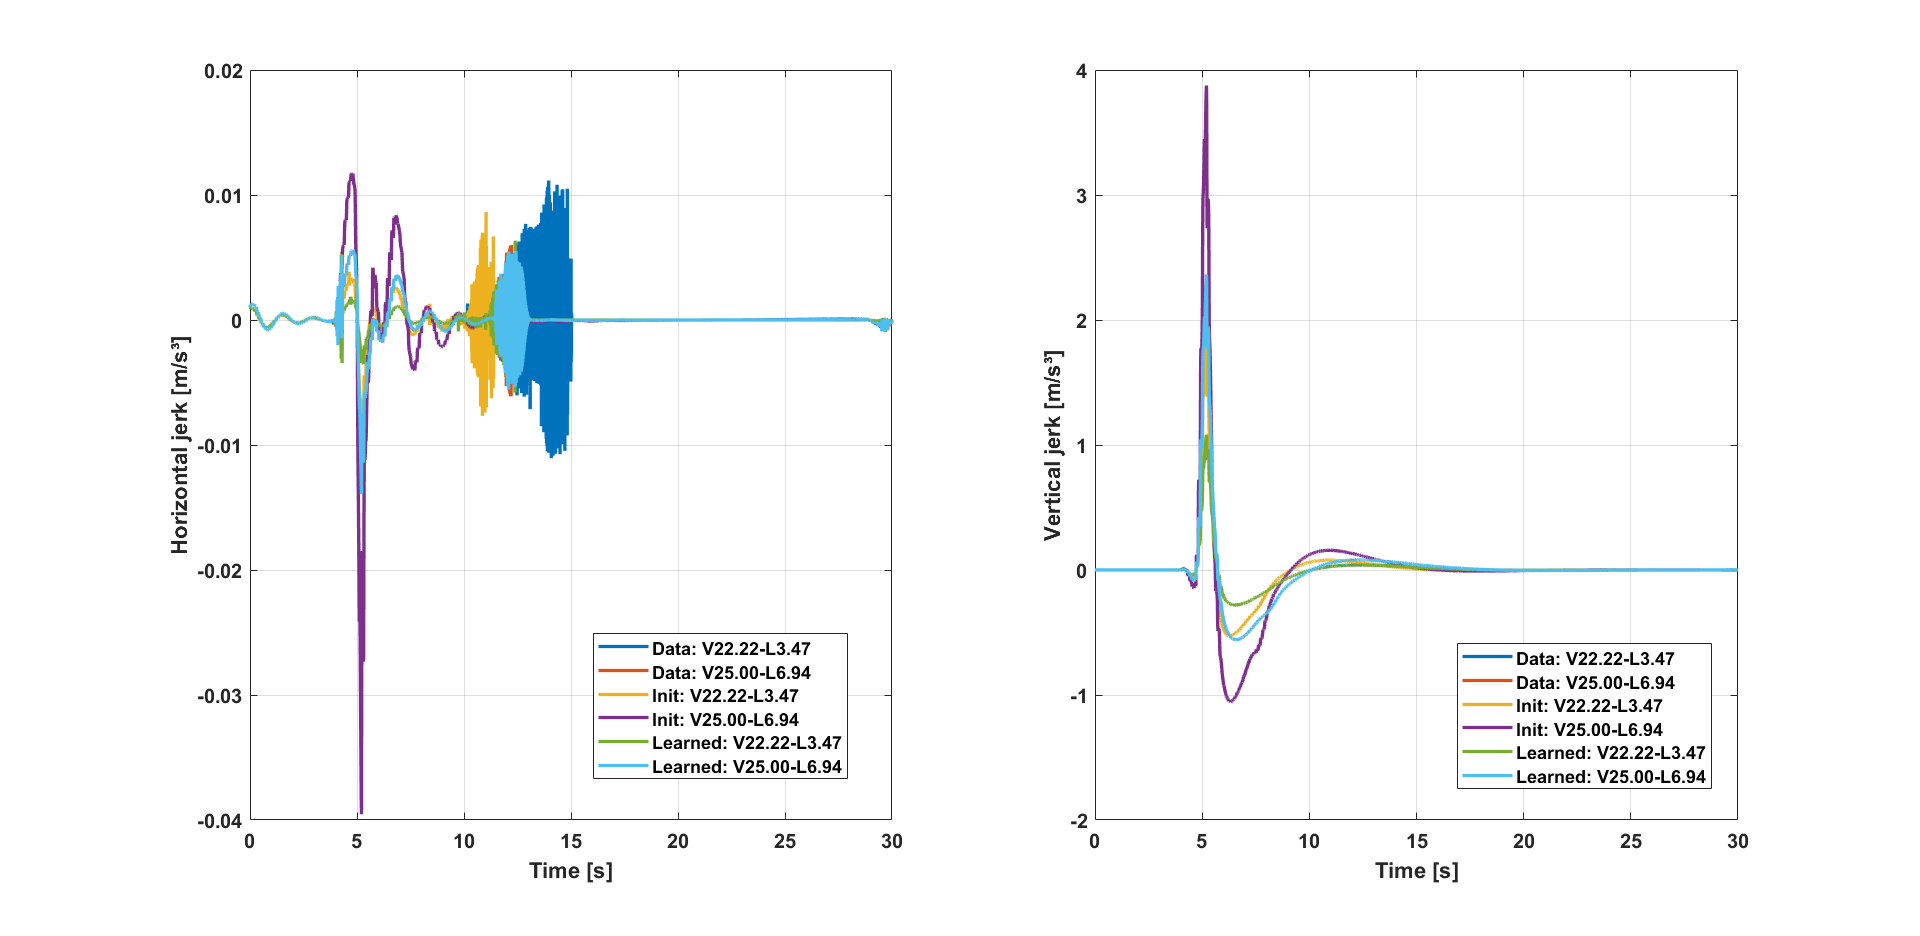
\includegraphics[width=1.1\textwidth]{7JX_JY_N1000IT28.PNG}
	\caption{This Figure shows the observed jerk signals, the initial solution retrieved with as weights an all one vector and the learned solution.}	
	\label{fig:complex_jerk}
\end{figure}
                                    
                    











\section{Conclusion}

%%% Local Variables: 
%%% mode: latex
%%% TeX-master: "thesis"
%%% End: 